\documentclass[class=elsarticle,tikz=true]{standalone}

\usepackage[utf8]{inputenc}

\usepackage[]{multirow}
%\usepackage{texstyles/tikz-cellular}
%\usepackage{texstyles/tikz-vcond}
%\usepackage{texstyles/tikz-extension}
\usetikzlibrary{%
	positioning,
	fit,
	calc,
	arrows,
	arrows.meta,
	shapes.misc
}
%\usetikzlibrary{arrows,arrows.meta}
%\usetikzlibrary{positioning,arrows,matrix,shapes.geometric,fit,calc}
%\usepackage{amssymb}
\begin{document}

	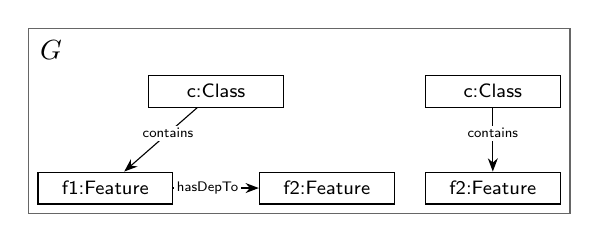
\begin{tikzpicture}[
		SClass/.style={draw,shape=rectangle,font=\sffamily,text width={width("rc=cc:Class")},align=center,inner xsep=-1pt},
	%	SClass-phantom/.style={text width={width(": Feature")},align=center,draw},
		title/.style={text width={width("$L_1R_2$")},inner sep=.5pt,outer sep=.5pt},
		outside/.style={draw=black!60}
	]
	
	
	
		
		%G
		\node(C32) [title] {$G$};
		\node(class32) [SClass, below right=15pt and 40pt of C32.west, anchor=west]{\scriptsize c:Class};
		\node (f1-C32) [SClass,below =50pt  of C32.west,anchor=west] {\scriptsize f1:Feature }  ;
		\node (f2-C32) [SClass,below right=50pt and 80pt of C32.west,anchor=west] {\scriptsize f2:Feature }  ;
		
		\draw [-{Stealth}] (class32)  to node [fill=white,inner sep=1pt,pos=.4,font=\sffamily] { \tiny contains }  (f1-C32);
		\draw [-{Stealth}] (f1-C32)  to node [fill=white,inner sep=1pt,pos=.4,font=\sffamily] { \tiny hasDepTo}  (f2-C32);
		
		\node(class2) [SClass,  right=100pt  of class32.west, anchor=west]{\scriptsize c:Class};	
		\node (f3) [SClass,below=35pt of class2.west,anchor=west] {\scriptsize f2:Feature }  ;
		\draw [-{Stealth}] (class2)  to node [fill=white,inner sep=1pt,pos=.4,font=\sffamily] { \tiny contains }  (f3);
		\node(C_32-out) [outside, fit={(C32) (f1-C32) (class32)(f2-C32) (class2) (f3)}]{};
	
		
		
	\end{tikzpicture}
	
%$\begin{array}{l} 
%\nexists \left( \tikz {% 
	%\node (cc1) [SClass] {\scriptsize rc2=cc1:Class }  ; 
	%\node (cc2) [SClass, strictly right of= cc1,node distance=4em] {\scriptsize rc1=cc2:Class }  ;
	%\node (cf1) [SClass, strictly below of= cc1,node distance=2em] {\scriptsize rf=cf1:Feature }  ;
	%\node (cf2) [SClass, strictly below of= cc2,node distance=2em] {\scriptsize cf2:Feature }  ;
	%\draw [-{Stealth}] (cc2)  to node [above,sloped] { \tiny contains }  (cf1)  ; 
	%\draw [-{Stealth}] (cc2)  to node [right] { \tiny contains }  (cf2)  ;
	%\draw [-{Stealth}] (cf1)  to node [above] { \tiny hasDepTo }  (cf2)  ;
%}  \right) 
%\land \, \nexists \left( \tikz {%
	%\node (cc1) [SClass] {\scriptsize rc2=cc1:Class }  ; 
	%\node (rc1) [SClass, strictly left of= cc1,node distance=2em] {\scriptsize rc1:Class }  ;
	%\node (cc2) [SClass, strictly right of= cc1,node distance=4em] {\scriptsize cc2:Class }  ;
	%\node (cf1) [SClass, strictly below of= cc1,node distance=2em] {\scriptsize rf=cf1:Feature }  ;
	%\node (cf2) [SClass, strictly below of= cc2,node distance=2em] {\scriptsize cf2:Feature }  ;
	%\draw [-{Stealth}] (rc1)  to node [above,sloped] { \tiny contains }  (cf1)  ; 
	%\draw [-{Stealth}] (cc2)  to node [right] { \tiny contains }  (cf2)  ;
	%\draw [-{Stealth}] (cf1)  to node [above] { \tiny hasDepTo }  (cf2)  ;
%}  \right) \land
%\vspace{4pt}
%\cr 
%\nexists \left( \tikz {%
	%\node (cc1) [SClass] {\scriptsize rc1=cc1:Class }  ; 
	%\node (cc2) [SClass, strictly right of= cc1,node distance=4em] {\scriptsize rc2=cc2:Class }  ;
	%\node (cf1) [SClass, strictly below of= cc1,node distance=2em] {\scriptsize cf1:Feature }  ;
	%\node (cf2) [SClass, strictly below of= cc2,node distance=2em] {\scriptsize rf=cf2:Feature }  ;
	%\draw [-{Stealth}] (cc1)  to node [left] { \tiny contains }  (cf1)  ; 
	%\draw [-{Stealth}] (cc1)  to node [above,sloped] { \tiny contains }  (cf2)  ;
	%\draw [-{Stealth}] (cf1)  to node [above] { \tiny hasDepTo }  (cf2)  ;
%}  \right) 
%\land \, \nexists \left( \tikz {%
	%\node (cc1) [SClass] {\scriptsize cc1:Class }  ; 
	%\node (rc1) [SClass, strictly right of= cc1,node distance=2em] {\scriptsize rc1:Class }  ;
	%\node (cc2) [SClass, strictly right of= cc1,node distance=6em] {\scriptsize rc2=cc2:Class }  ;
	%\node (cf1) [SClass, strictly below of= cc1,node distance=2em] {\scriptsize cf1:Feature }  ;
	%\node (cf2) [SClass, strictly below of= cc2,node distance=2em] {\scriptsize rf=cf2:Feature }  ;
	%\draw [-{Stealth}] (rc1)  to node [above,sloped] { \tiny contains }  (cf2)  ; 
	%\draw [-{Stealth}] (cc1)  to node [right] { \tiny contains }  (cf1)  ;
	%\draw [-{Stealth}] (cf1)  to node [above] { \tiny hasDepTo }  (cf2)  ;
%}  \right) \land
%\vspace{4pt}
%\cr 
%\nexists \left( \tikz {%
	%\node (cc1) [SClass] {\scriptsize rc1=cc1:Class }  ; 
	%\node (cc2) [SClass, strictly right of= cc1,node distance=4em] {\scriptsize rc2=cc2:Class }  ;
	%\node (cf1) [SClass, strictly below of= cc1,node distance=2em] {\scriptsize cf1:Feature }  ;
	%\node (cf2) [SClass, strictly below of= cc2,node distance=2em] {\scriptsize cf2:Feature }  ;
	%\node (cf3) [SClass, strictly left of= cf1,node distance=4em] {\scriptsize rf=cf3:Feature }  ;
	%\draw [-{Stealth}] (cc2)  to node [left] { \tiny contains }  (cf2)  ; 
	%\draw [-{Stealth}] (cc1)  to node [above,sloped] { \tiny contains }  (cf3)  ;
	%\draw [-{Stealth}] (cc1)  to node [right] { \tiny contains }  (cf1)  ;
	%\draw [-{Stealth}] (cf1)  to node [above] { \tiny hasDepTo }  (cf2)  ;
	%\draw [-{Stealth}] (cf1)  to node [above] { \tiny hasDepTo }  (cf3)  ;
 %}  \right) 
%\land \, \nexists \left( \tikz {%
	%\node (cc1) [SClass] {\scriptsize rc1=cc1:Class }  ; 
	%\node (cc2) [SClass, strictly right of= cc1,node distance=4em] {\scriptsize cc2:Class }  ;
	%\node (rc2) [SClass, strictly left of= cc1,node distance=4em] {\scriptsize rc2:Class }  ;
	%\node (cf1) [SClass, strictly below of= cc1,node distance=2em] {\scriptsize cf1:Feature }  ;
	%\node (cf2) [SClass, strictly below of= cc2,node distance=2em] {\scriptsize cf2:Feature }  ;
	%\node (cf3) [SClass, strictly left of= cf1,node distance=4em] {\scriptsize rf=cf3:Feature }  ;
	%\draw [-{Stealth}] (cc2)  to node [left] { \tiny contains }  (cf2)  ; 
	%\draw [-{Stealth}] (cc1)  to node [above,sloped] { \tiny contains }  (cf3)  ;
	%\draw [-{Stealth}] (cc1)  to node [right] { \tiny contains }  (cf1)  ;
	%\draw [-{Stealth}] (cf1)  to node [above] { \tiny hasDepTo }  (cf2)  ;
	%\draw [-{Stealth}] (cf1)  to node [above] { \tiny hasDepTo }  (cf3)  ;
%}  \right)
%\end{array}$
\end{document}